% Author: Max Melching, 2025
% With elements from https://tikz.net/hyperbola/
\documentclass[border=3pt,tikz]{standalone}


\usepackage{tikz}
\usepackage{pgfplots} % for the axis environment
\usepackage[outline]{contour}
\usepackage{xcolor}
\usepackage{newtxmath}  % Use Times in math mode
\usepackage{tgpagella}  % Use Pagella in text


\colorlet{mydarkred}{red!70!black}
\colorlet{mydarkgreen}{green!40!black}


\usetikzlibrary{arrows.meta, calc, decorations.markings}
\pgfplotsset{compat=1.11}  % Make "axis cs" default coordinate system in axis
% \pgfplotsset{compat=1.16}  % Make "axis cs" default coordinate system in axis


\tikzset{
    >={Stealth[inset=0,angle'=27]},
    mass/.style={
        mydarkred,
        fill,
    },
    trajectory/.style={
        mydarkgreen,
        % thick,
        line width=0.8,
        % postaction=decorate,
        % decoration={
        %     markings,
        %     mark=between positions 0.01 and 1 step 0.1 with \arrow{>}
        %     % mark=at position 0.25 with \arrow{>}
        % },
    },
}



\begin{document}


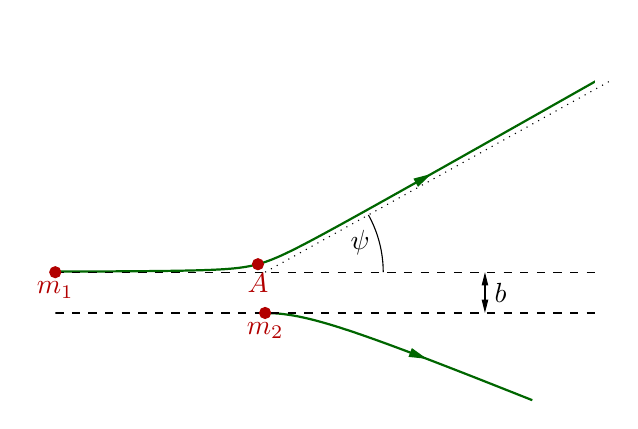
\begin{tikzpicture}[scale=1]
    % limits & parameters
    \def\xa{-35}
    \def\xb{55}
    \def\ya{-20}
    % \def\yb{55}
    \def\yb{35}
    \def\tmax{4}
    \def\N{30} % number of points

    
    \def\a{1}  % Force strength basically
    \def\b{5}
    \def\c{sqrt(\a^2+\b^2)}

    \def\atwo{10}
    \def\btwo{3}
    \def\tmaxtwo{2.2}
    \def\Ntwo{10} % number of points

    
    \begin{axis}[
        xmin=\xa,
        xmax=\xb,
        ymin=\ya,
        ymax=\yb,
        hide x axis,
        hide y axis,
    ]
        \addplot[
            trajectory,
            postaction=decorate,
            decoration={
                markings,
                mark=at position 0.6 with \arrow{>},  % Error for most other values
            },
            smooth,
            samples=\N,
            variable=\t,
            domain=-\tmax:\tmax,
        ] ({\a/\c*(-\a*cosh(\t)-\c) + \b/\c*\b*sinh(\t)},
           {-\b/\c*(-\a*cosh(\t)-\c) + \a/\c*\b*sinh(\t)});

        \draw[
            trajectory,
            postaction=decorate,
            decoration={
                markings,
                mark=at position 0.6 with \arrow{>},
            },
            smooth,
            samples=\Ntwo,
            variable=\t,
            domain=0:\tmaxtwo,
        ] plot({\atwo*sinh(\t)},{-\btwo*cosh(\t)+\btwo});


        \coordinate (m1) at (\xa, \b);
        \coordinate (m2) at (0, 0);


        \draw[
            dashed,
        ] (\xa, \b) -- (\xb, \b);

        \draw[
            dashed,
        ] (\xa, 0) -- (\xb, 0);
        
        \draw[
            % dashed,
            <->,
            % thick,
        ] (2*\xb/3, 0) -- (2*\xb/3, \b) node[midway, right] {$b$};


        \coordinate (A) at ({\a/\c*(-\a*cosh(0)-\c) + \b/\c*\b*sinh(0)}, {-\b/\c*(-\a*cosh(0)-\c) + \a/\c*\b*sinh(0) });

        \coordinate (scatangle) at (0, \b);
        
    \end{axis}


    % -- Circle cannot be drawn in axis environment, thus do here
    \draw[mass] (m1) circle (0.07) node[below] {$m_1$};
    \draw[mass] (m2) circle (0.07) node[below] {$m_2$};

    \draw[mass] (A) circle (0.07) node[below] {$A$};
    

    \def\psival{29}

    \draw[
        dotted,
    ] (scatangle) --++ (\psival:5);
    
    \def\arcradius{1.5}
    % \draw[thick] (29:1) arc(29:-29:1);
    \draw (scatangle)++(\psival:\arcradius) arc(\psival:0:\arcradius) node[midway, left] {$\psi$};


    % \def\thetaval{-21}

    % \draw[
    %     dotted,
    % ] (scatangle) --++ (\thetaval:5);
    
    % \draw[
    %     dotted,
    % ] (m2) --++ (\thetaval:5);

    % \def\arcradius{2}
    % \draw (scatangle)++(\psival:\arcradius) arc(\psival:\thetaval:\arcradius) node[midway, left] {$\theta$};
    % TODO: this is not theta. We must draw from position of m2 at time t to m1 at time t

\end{tikzpicture}



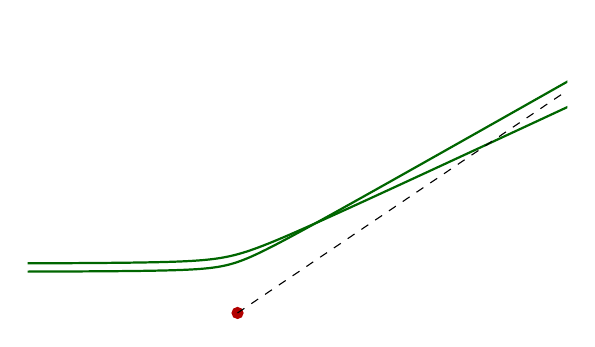
\begin{tikzpicture}[scale=1]
    % limits & parameters
    \def\xa{-35}
    \def\xb{55}
    \def\ya{-20}
    % \def\yb{ 55}
    \def\yb{35}
    \def\tmax{4}
    \def\N{30} % number of points

    
    \def\a{1}  % Force strength basically
    \def\b{5}
    \def\c{sqrt(\a^2+\b^2)}

    \def\atwo{10}
    \def\btwo{3}
    \def\tmaxtwo{2.2}
    \def\Ntwo{10} % number of points

    
    \begin{axis}[
        xmin=\xa,
        xmax=\xb,
        ymin=\ya,
        ymax=\yb,
        hide x axis,
        hide y axis,
    ]
        \foreach \b in {5, 6} {
            \addplot[
                trajectory,
                % postaction=decorate,
                % decoration={
                %     markings,
                %     mark=at position 0.6 with \arrow{>},  % Error for most other values -> ah, only works for b=5
                % },
                smooth,
                samples=\N,
                variable=\t,
                domain=-\tmax:\tmax,
            ] ({  \a/\c*(-\a*cosh(\t)-\c) + \b/\c*\b*sinh(\t) },
            { -\b/\c*(-\a*cosh(\t)-\c) + \a/\c*\b*sinh(\t) });
        }


        \coordinate (m2) at (0, 0);
    \end{axis}


    % -- Circle cannot be drawn in axis environment, thus do here
    \draw[mass] (m2) circle (0.07);% node[below] {$m_2$};
    
    \draw[
        dashed,
    ] (m2) --++ (34:5);
    % TODO: is origin the scattering center?
    % -> angle looks odd here

\end{tikzpicture}
% TODO: also careful here, is analysis from CMS!!! Unlike first plot


\end{document}